\documentclass{article}
\addtolength{\oddsidemargin}{-.875in}
\addtolength{\evensidemargin}{-.875in}
\addtolength{\textwidth}{1.0in}
\addtolength{\topmargin}{-0.5in}
\addtolength{\textheight}{1.00in}
\usepackage{wrapfig}
\usepackage{sidecap}
\usepackage{hyperref}
\usepackage[pdftex]{graphicx}
\usepackage[utf8]{inputenc}
\usepackage[spanish]{babel}

\title{Reporte de Actividades - Enero 2015 - Diciembre 2018}
\author{Jaime E. Forero Romero\\Profesor Asociado - Departamento de
  F\'isica\\Universidad de los Andes}  
\begin{document}

\maketitle
\tableofcontents
\newpage

\section{Docencia}

\subsection{Cursos dictados}
\begin{tabular}{p{6.5cm} l c c}\hline
Curso & Semestre & Inscritos\\\hline
F\'isica I & 2018-20 &  47 \\
M\'etodos Computacionales Avanzados & 2018-20 &   31 \\\hline
F\'isica I & 2018-10 &   60\\
M\'etodos Computacionales & 2018-10 &  24 \\
Taller de Astronom\'ia & 2018-10 &  23 \\\hline
STAI & 2017-20 & - \\\hline
F\'isica II & 2017-10 & 68 \\
M\'etodos Computacionales Avanzados & 2017-10 & 17 \\ 
Taller de Astronom\'ia & 2017-10 & 19 \\\hline
Astronom\'ia Popular (CBU) & 2016-10 & 92 \\
M\'etodos Computacionales & 2016-20 & 20 \\
Taller de Astronom\'ia & 2016-20 & 14 \\\hline
F\'isica I & 2016-10 & 80 \\
M\'etodos Computacionales Avanzados & 2016-10 & 9 \\
Taller de Astronom\'ia & 2016-10 & 6 \\\hline
Astronom\'ia Popular (CBU) & 2015-20 & 91 \\ 
M\'etodos Computacionales & 2015-20 & 10 \\
Taller de Astronom\'ia & 2015-20 & 70 \\\hline
F\'isica I & 2015-10 & 96 \\
Electromagnetismo II & 2015-10 & 6  \\
Taller de Astronom\'ia & 2015-10 & 10 \\\hline
Total Estudiantes & & 793 & \\\hline
\end{tabular}

\subsection{Desarrollo de nuevos cursos}
\begin{itemize}
\item Construcci\'on de un nuevo CBU: \emph{Astronom\'ia Popular}.

Programa:

\url{https://github.com/forero/AstronomiaPopular/blob/master/syllabus/ProgramaCBU_AstronomiaPopular.pdf}

\item Construcci\'on de un nuevo curso para pregrado avanzado y
  posgrado: \emph{M\'etodos Computacionales Avanzados}.

Programa:

\url{https://github.com/ComputoCienciasUniandes/MetodosComputacionalesAvanzados/blob/master/syllabus/syllabus.pdf}
\item Re-estructuraci\'on del curso \emph{Herramientas Computacionales} en
  una metodolog\'ia \emph{flipped-classroom}.
Esto implic\'o la creaci\'on de una serie de 15 videos con una
duraci\'on total cercana a las 5 horas de contenidos en reproducci\'on
continua.  
En promedio cada video ha sido visto 2000 veces en youtube.
Con cerca de 30000 vistas en total, el curso estaría en el top 40 de
videos con más vistas del canal institucional de Uniandes. 
Cada video tiene más vistas que el 80$\%$ de todos los videos del canal
institucional de Uniandes.

Programa:

\url{https://github.com/ComputoCienciasUniandes/HerramientasComputacionales/blob/master/Syllabus/Syllabus.pdf}    

Lista de videos:

\url{https://www.youtube.com/playlist?list=PLHQtzvthdVM_MGC9dPFKe4hPAwBd_7RJ3} 

\item Re-estructuraci\'on de un curso para estudiantes de todas las
  carreras: \emph{Taller de Astronom\'ia}. 
Este curso de un cr\'edito fue creado depu\'es de detectar la
necesidad de ofrecer un curso que diera una introducci\'on a la
astronom\'ia. 
Durante el curso se balancean charlas de temas b\'asicos de
astronom\'ia, explicaci\'on de noticias recientes relacionadas con
astronom\'ia y presentaciones de investigadores nacionales hechas a un
nivel divulgativo. 

\end{itemize}



\subsection{Educaci\'on Continuada}
\begin{itemize}
\item Abril 2017. Una adaptaci\'on del curso Herramientas Computacionales fu\'e
  dictada como un curso abierto y gratuito para estudiantes de
  Uniandes y otras universidades. El evento se llam\'o Python Bootcamp
  y se dict\'o en 16 horas de clase en dos d\'ias. El curso cont\'o
  con 100 asistentes. \url{https://pythonbootcampuniandes.github.io/}
\item Agosto 2016. Una adaptaci\'on del CBU Astronom\'ia Popular se dict\'o como
  curso de 16 horas a trav\'es de Educaci\'on Continuada de
  Uniandes. El curso cont\'o con 10 asistentes.
\end{itemize}

\subsection{Escuelas Internacionales}
\begin{itemize}

\item {Julio 2018. Instructor y co-organizador de la 41 edici\'on de
  la International School for Young Astronomers de la Uni\'on
  Astron\'omica Internacional (3 semanas de duraci\'on, 8 instructores
  internacionales, 30 estudiantes latinamericanos). 

\url{https://eventos.redclara.net/indico/event/842/}. }

\item {Junio 2015. Organizador de la una escuela Andina de
  Cosmolog\'ia (1 mes de duraci\'on, 4 instructores internacionales,
  20 estudiantes de la regi\'on andina). 

\url{http://www.astro4dev.org/blog/category/tf1/andean-cosmology-school/}. }
\end{itemize}

\subsection{Presentaciones Divulgativas}

\begin{tabular}{p{1.7cm} p{1.2cm} p{2.0cm} p{5.0cm} p{4.5cm}}\hline
Date & Country & City& Venue& Title\\\hline

3-02-2018 & Colombia & Santa Rosa de Cabal & Minkalab & Ubicaci\'on
espacial y temporal en el Universo\\
27-01-2017 & Colombia & Bogot\'a & Liceo Franc\'es & Generalidades de Astrof\'isica y Cosmolog\'ia\\
19-02-2016 & Colombia & Medell\'in & Planetario de Medell\'in & Tiempos Cosmol\'ogicos\\
18-02-2016 & Colombia & Medell\'in & OPUS - Oficina de Arquitectura & Tiempos Cosmol\'ogicos\\
8-10-2015  & Colombia & Bogot\'a & Universidad Santo Tom\'as & Vida Cosmol\'ogica \\
21-05-2015 & Colombia & Bogot\'a & Conversatorio Maloka & De d\'onde vengo yo. Luz, estrellas y galaxias.\\
11-03-2015 & Colombia & B/manga & Caf\'e Cient\'ifico & Cielos Fluidos y Astronom\'ia Perif\'erica. Dos proyectos de Arte y Astronom\'ia.\\\hline
\end{tabular}

\subsection{Aparici\'on en medios de comunicaci\'on}

\begin{itemize}
\item Noviembre 2018. Entrevista sobre el proyecto DESI publicada en El Tiempo:

 \url{http://www.eltiempo.com/vida/ciencia/atlas-3d-mas-completo-del-universp-155450}.
\end{itemize}

\subsection{Direcci\'on de monograf\'ia de pregrado}

\begin{itemize}
\item [10] Javier Acevedo, \emph{Simulating collisional dark matter using a
  Lattice Boltzmann method}, 2018-20.  
\item [9] Sergio Lobo, \emph{Recovery of DESI BGS redshift
  measurements using Machine Learning}. 2018-20.  
\item [8] David Paipa, \emph{Supercluster characterization in
  cosmological simulations}. 2018-20. 
\item [7] Sebasti\'an Sanabria, \emph{Dark matter halo dynamics in the
  cosmic web}. 2018-10. 
\item [6] Sebastian Franco Ulloa, \emph{Simulaciones de un fluido
  débilmente auto-interactuante con métodos Lattice-Boltzmann},
  2017-10
\item [5] Nicol\'as Romero, \emph{Observational evidence of star formation
  stochasticity in the CALIFA dataset}, 2016-20.
\item [4] David Bernal, \emph{Acotando las velocidades tangenciales de las
  galaxias satélites de Andrómeda utilizando optimización no lineal}, 2016-20.
\item [3] Sergio Hernandez Charpak, \emph{Laniakea in a Cosmological
  Context or Detection of Galaxy Superclusters in Simulated
  Cosmological Structures}, 2016-10
\item [2] Mar\'ia Camila Remolina Guti\'errez, \emph{Influence of galaxy
  rotation and outflows in the Lyman Alpha spectral line}, 2015-20
\item [1] Christian Poveda, \emph{A Semi-Analytic Approach to Formation
  Processes in Galaxies}, 2015-10
\end{itemize}


\newpage
\section{Investigaci\'on}

\subsection{Refereed Papers}

En subrayado sencillo se encuentran estudiantes de pregrado de
Uniandes, en subrayado doble se encuentran postdocs de Uniandes.

\begin{itemize}

\item[10]{\it Unbiased clustering estimates with the DESI fibre
  assignment}. 

D. Bianchi, A. Burden,  W. J. Percival, D. Brooks,
R. N. Cahn, {\bf J. E. Forero-Romero}, M. Levi, A. J. Ross, G. Tarle.

Monthly Notices of the Royal Astronomical Society, Volume 481, Issue
2,

\url{https://doi.org/10.1093/mnras/sty2377}

\item[9]{\it We are not the 99 percent: quantifying asphericity in the
  distribution of Local Group satellites}.

{\bf J. E. Forero-Romero}, \underline{\underline{V. Arias}}.

Monthly Notices of the Royal Astronomical Society, Volume 478, Issue
4, 

\url{https://doi.org/10.1093/mnras/sty1349}

\item[8]{\it Modelling the gas kinematics of an atypical Lyman alpha
emitting compact dwarf galaxy}.

{\bf J. E. Forero-Romero}, M. Gronke,
  \underline{M. C. Remolina-Guti\'errez}, N. Garavito-Camargo, M. Dijkstra.

  Monthly Notices of the Royal Astronomical Society, Volume 474, Issue
  1, 2018. 

\url{https://doi.org/10.1093/mnras/stx2699}.  

\item[7]{\it Tracing the cosmic web}.

N. I. Libeskind, R. van de
  Weygaert, M. Cautun, B. Falck, E. Tempel, T. Abel, M. Alpaslan, M. A. Aragón-Calvo, {\bf
  J. E. Forero-Romero},  R. Gonzalez, S. Gottl\"ober, O. Hahn 13 ,
W. A. Hellwing, Y. Hoffman, B. J. T. Jones, F. Kitaura, A. Knebe,
S. Manti, M. Neyrinck, S. E. Nuza, N. Padilla, E. Platen,
N. Ramachandra, A. Robotham, E. Saar, S. Shandarin, M. Steinmetz,
R. S. Stoica, Th. Sousbie, G. Yepes.

Monthly Notices of the Royal Astronomical Society, Volume 473, Issue
1, 2018. 

\url{https://doi.org/10.1093/mnras/stx1976}. 

\item[6]{\it Boosting Lya and HeII 1640A Line Fluxes from Pop III
  Galaxies: Stochastic IMF Sampling and Departures from
  Case-B}. 

L. Mas-Ribas, M. Dijkstra, {\bf J.E. Forero-Romero}.

The Astrophysical Journal, Volume 833, Issue 1, 2016. 

\url{https://doi.org/10.3847/1538-4357/833/1/65}. 


\item[5]{\it Quantifying and controlling biases in dark matter halo
  concentration estimates}, 

\underline{C.N. Poveda-Ruiz}, {\bf J.E. Forero-Romero}, J.C. Mu\~noz-Cuartas. 

The Astrophysical Journal, Volume 832, Issue 2, 2016. 

\url{https://doi.org/10.3847/0004-637X/832/2/169}.

\item[4]{\it Impact of Cosmic Variance on the Galaxy-Halo Connection
  for Lyman-$\alpha$ emitters}.  

J.E. Mej\'ia-Restrepo, {\bf J.E. Forero-Romero}.

The Astrophysical Journal, Volume 828, Issue 1.

\url{https://doi.org/10.3847/0004-637X/828/1/5}.

\item[3]{\it SPOKES: An end-to-end simulation facility for
  spectroscopic cosmological surveys}.
 
	Nord, B.; Amara, A.; R\'efr\'egier, A.; Gamper, La.; Gamper, Lu.;
        Hambrecht, B.; Chang, C.; {\bf Forero-Romero, J. E.}; Serrano, S.;
        Cunha, C.; Coles, O.; Nicola, A.; Busha, M.; Bauer, A.;
        Saunders, W.; Jouvel, S.; Kirk, D.; Wechsler, R.

Astronomy and Computing, Volume 15, p. 1-15, 2016.

\url{https://doi.org/10.1016/j.ascom.2016.02.001}.

\item[2]{\it The Local Group in the Cosmic Web}.

{\bf J.E. Forero-Romero}, R. González.

The Astrophysical Journal, Volume 799, Issue 1, 2015.

\url{https://doi.org/10.1088/0004-637X/799/1/45}.

\item[1] {\it Tensor anisotropy as a tracer of cosmic voids}. 

S. Bustamante, {\bf J.E. Forero-Romero}. 

Monthly Notices of the Royal Astronomical Society, Volume 453, Issue 1, 2015.

\url{https://doi.org/10.1093/mnras/stv1637}.

\end{itemize}

\subsection{Non-Refereed Papers}

\begin{itemize}

\item[2] 
{\it The DESI Experiment Part II: Instrument Design}. 

The DESI Collaboration. 

\url{http://adsabs.harvard.edu/abs/2016arXiv161100037D}.


\item[1] 
{\it The DESI Experiment Part I: Science,Targeting, and Survey
  Design}. 

The DESI Collaboration. 

\url{http://adsabs.harvard.edu/abs/2016arXiv161100036D}.




\end{itemize}


\subsection{Conference Proceedings}

\begin{itemize}

\item[5]{\it Looking for observational evidence of star formation
  stochasticity in the CALIFA dataset}.
	
\underline{N. Romero-Díaz},  {\bf J.E. Forero-Romero}.

XV Latin American Regional IAU Meeting Cartagena 2016, Revista Mexicana
de Astronomía y Astrofísica (Serie de Conferencias) Vol. 49,
pp. 110-110, 2017.

\item[4]{\it Cosmology with the cosmic web}.

{\bf J.E. Forero-Romero}.

XV Latin American Regional IAU Meeting Cartagena 2016, Revista Mexicana
de Astronomía y Astrofísica (Serie de Conferencias) Vol. 49,
pp. 119-119, 2017.

\item[3]{\it Laniakea in a Cosmological Context}.


\underline{S.D. Hernandez-Charpak}, {\bf J.E. Forero-Romero}.

XV Latin American Regional IAU Meeting Cartagena 2016, Revista Mexicana
de Astronomía y Astrofísica (Serie de Conferencias) Vol. 49,
pp. 123-123, 2017.


\item[2] {\it The influence of environment on the HI mass functions in
  cosmological simulations}.
 
\underline{J.D. Prada-Gonzalez}, M. G. Jones, {\bf J.E. Forero-Romero}, M.P. Haynes.

XV Latin American Regional IAU Meeting Cartagena 2016, Revista Mexicana
de Astronomía y Astrofísica (Serie de Conferencias) Vol. 49,
pp. 132-132, 2017.

\item [1] {\it Influence of galaxy rotation and outflows on the Lyman
  Alpha spectral line}. 
	
\underline{M.C. Remolina-Gutiérrez}, {\bf J.E. Forero-Romero},
J.N. Garavito-Camargo.

XV Latin American Regional IAU Meeting Cartagena 2016, Revista Mexicana
de Astronomía y Astrofísica (Serie de Conferencias) Vol. 49,
pp. 135-135, 2017.
\end{itemize}


\subsection{Rankings de citaciones}
\begin{figure}[!h]
\begin{center}
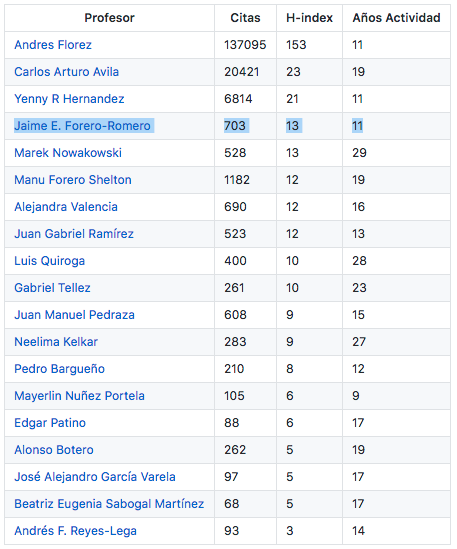
\includegraphics[scale=0.5]{scholar_fisica.png}
\caption{
El impacto de mi producci\'on investigativa se clasifica en el {\bf cuartil
  superior de los profesores de planta del departamento de F\'isica} en
  un ranking decreciente por H-index. 
  En esta clasificaci\'on se toman en cuenta los resultados de
  perfiles p\'ublicos de Google Scholar
  para los \'ultimos cinco a\~nos de citaciones solamente, esto con el
  inter\'es de descontar el efecto de investigadores con m\'as a\~nos de
  actividad y comparar con mejor paridad la productividad
  reciente. Esta tabla se encuentra en: \url{https://github.com/forero/gsc/blob/master/info/fisica_uniandes.md}\label{table:fisica}}
\end{center}
\end{figure}

\newpage

\begin{figure}[!h]
\begin{center}
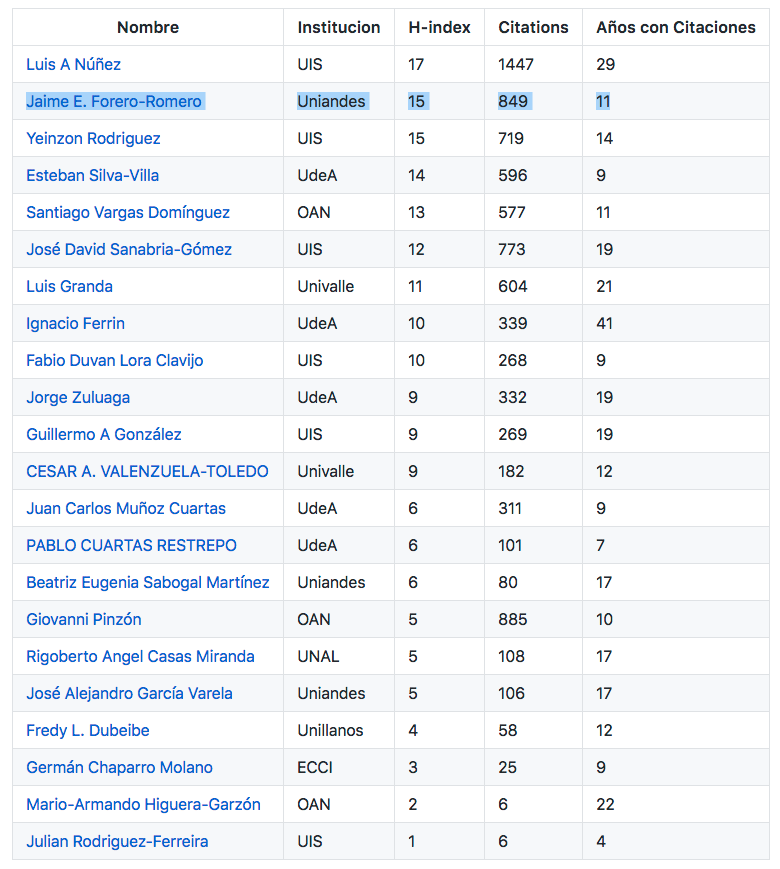
\includegraphics[scale=0.5]{scholar_astronomia.png}
\caption{
El impacto de mi producci\'on investigativa se clasifica en el {\bf cuartil
  superior de todos los investigadores colombianos en el \'area de
  astronom\'ia y astrof\'isica} en 
  un ranking decreciente por H-index. 
  En esta clasificaci\'on se toman en cuenta los resultados de
  perfiles p\'ublicos de Google Scholar
  para los \'ultimos cinco a\~nos de citaciones solamente, esto con el
  inter\'es de descontar el efecto de investigadores con m\'as a\~nos de
  actividad y comparar con mejor paridad la productividad
  reciente. 
Esta tabla se encuentra en: 
\url{https://github.com/ColombianAstronomy/ProductividadAstronomica/blob/master/google_scholar.md}
\label{table:astro}}
\end{center}
\end{figure}

\newpage

\subsection{Asesor\'ia posgrado}

Doctorado:
\begin{itemize}
\item [1] Diego Barbosa. Presentar\'a examen de candidatura a finales 2019-10.
\item [2] John Fredy Su\'arez. Ya vi\'o materias. Presentar\'a examen
  de conocimientos en 2019-20.
\item [3] Yeimy Camargo, \emph{Galaxy Formation Bias in the Cosmic
  Web}. En curso. Estudiante de doctorado en la Universidad Nacional de Colombia
  Sede Bogot\'a. Soy su co-director.
\end{itemize}

Maestr\'ia:
\begin{itemize}
\item [3] Felipe G\'omez, \emph{A Large Scale Structure Void
  Identifier based on $\beta$-Skeleton}, en curso.
\item [2] Jes\'us Prada, \emph{The shape of the Milky Way Dark Matter
  Halo}, 2018-10.
\item [1] Juan Nicol\'as Garavito, \emph{The effect of gas bulk rotation
  on the morphology of the Lyman alpha line}, 2015-20.
\end{itemize}


\subsection{Asesor\'ia de postdocs}

\begin{itemize}
\item Ver\'onica Arias. 2015-2016. Como resultado principal tenemos
  una publicaci\'on en una revista internacional de primer cuartil.

\end{itemize}

\subsection{Financiaci\'on}
\begin{tabular}{l l l p{2.4cm} p{4.0cm} c}\hline
N$^{o}$ & Fecha & Duraci\'on & Instituci\'on & Proyecto & Monto \\\hline
1 & 1.10.2016 & 36 meses & COLCIENCIAS & Simulaciones y Observaciones del Universo a Gran Escala & 200 Millones COP\\\hline
2 & 1.03.2017 & 48 meses & Uni\'on Europea & Latin-American Galaxy Formation Network \url{https://www.lacegal.com/} & 1.4 Millones EURO \\\hline
3 & 1.10.2017 & 24 meses & Uniandes & 
Spatio-Temporal Transient Object Localization in Astronomical Image
Sequences Using Machine Learning & 84 Millones COP \\
\\\hline 
\end{tabular}

\subsection{Visitas de investigaci\'on}
\begin{tabular}{p{1.7cm} p{1.3cm} p{2.0cm} p{1.5cm} p{7.0cm}}\hline
Date & Duration & Country & City & Institute\\\hline
18-11-2017 & 2 weeks & USA & Berkeley & Lawrence Berkeley National Laboratory\\
4-11-2017 & 2 weeks & USA & Honolulu & Institute for Astronomy\\
1-10-2017 & 5 weeks & South Korea & Daejeon & Korea Astronomy and Space Science Institute \\
26-09-2017 & 5 weeks & Germany & Heidelberg & Heidelberg Institute for Theoretical Studies\\
1-07-2017 & 5 weeks & UK & Durham & Institute for Computational Cosmology\\
25-07-2016 & 1 week & USA & Berkeley & Lawrence Berkeley National Laboratory\\
4-07-2016 & 1 week & Germany & Heidelberg & Heidelberg Institute for Theoretical Studies \\
27-06-2016 & 1 week & Germany & Potsdam & Leibniz Institute for Astrophysics \\
14-12-2015 & 1 week & Chile & Santiago & Pontificia Universidad Cat\'olica\\
25-10-2015 & 1 week & USA & Berkeley & Lawrence Berkeley National Laboratory\\
12-07-2015 & 2 weeks & UK & Durham & Durham University\\\hline
\end{tabular}

\subsection{Charlas t\'ecnicas y presentaciones en congresos}


\subsection*{2018}
\noindent
\begin{tabular}{p{2.0cm} p{1.5cm} p{1.5cm} p{4.5cm} p{6.0cm}}\hline
Date & Country & City& Venue & Title\\\hline
15-16-2018 & Per\'u & Lima & Coloquio de F\'isica Pontificia Universidad Cat\'olica & Construyendo el mapa 3D m\'as grande del Universo. \\
14-11-2018 & Per\'u & Lima & Tercer Workshop Astronom\'ia en los Andes & Astronom\'ia para el Desarrollo. \\
31-10-2018 & Colombia & Bogot\'a & II Workshop in Current Challenges in Cosmology & The Dark Energy Spectroscopic Instrument. \\
\end{tabular}

\subsection*{2017}
\noindent
\begin{tabular}{p{2.0cm} p{1.5cm} p{1.5cm} p{5.0cm} p{5.0cm}}\hline
Date & Country & City& Venue & Title\\\hline
15-12-2017 & Argentina & Bariloche & Meeting Distant Galaxies from the
Far South & Boosting the Lyman-alpha line from stochastic IMF sampling\\
13-11-2017 & USA & Honolulu & Extragalactic Astronomy Seminar at the Institute for Astronomy & We are not the 99\%: the Local Group in a Cosmological Context\\
19-10-2017 & South Korea & Daejeon & Cosmology Group Seminar at KASI & Simulating the Dark Energy Spectroscopic Instrument\\
10-02-2017 & Colombia & Bogot\'a & Pycon 2017 Colombia & Mapping the Universe with Python\\
\end{tabular}

\subsection*{2016}
\noindent
\begin{tabular}{p{2.0cm} p{1.5cm} p{1.5cm} p{5.0cm} p{5.0cm}}\hline
Date & Country & City& Venue & Title\\\hline
3-10-2016 & Colombia & Cartagena & XV Latinamerican Regional IAU Meeting & Cosmology with the Cosmic Web\\
29-06-2016 & Germany & Potsdam & Cosmology Group Seminar at the Leibniz Institute for Astrophysics & The Local Group, LAEs and the Cosmic Web\\
20-06-2016 & UK & Durham & DESI collaboration meeting & How to simulate DESI with Python\\
19-02-2016 & Colombia & Medell\'in & Universidad de Antioquia & Galaxias y la red c\'osmica\\
\end{tabular}

\subsection*{2015}
\noindent
\begin{tabular}{p{2.0cm} p{1.5cm} p{1.5cm} p{5.0cm} p{5.0cm}}\hline
Date & Country & City& Venue & Title\\\hline
18-12-2015 & Chile & Santiago & Pontificia Universidad Cat\'olica& Galaxias y la red c\'osmica \\
\end{tabular}


\subsection{Colaboraciones Internacionales de Alto Impacto}

\begin{itemize}

\item Dark Energy Spectroscopic Instrument (DESI).

Proyecto de \'ultima generaci\'on de cosmolog\'ia observacional.
El proyecto tiene un costo de hardware de 50 millones de d\'olares y
empezar\'a a tomar mediciones en el periodo 2019-2024.
El proyecto es liderado por Lawrence Berkeley National Laboratory
(Berkeley Lab). 
La colaboraci\'on incluye cerca de 465 investigadores de 70
instituciones diferentes en todo el mundo.
Uniandes hace parte formal de la colaboraci\'on desde el 2014 a
trav\'es de mis contactos desde la \'epoca en la que fu\'i postdoc en
Berkeley. 
{\bf Es la primera vez que Colombia} hace parte de un proyecto internacional
de frontera en cosmolog\'ia observacional.


Un press release reciente de Berkeley Lab
dice\footnote{\url{https://newscenter.lbl.gov/2018/02/12/solving-the-dark-energy-mystery-a-new-assignment-for-a-45-year-old-telescope/}}: 
\begin{quote}
“Installing DESI on the Mayall will put the telescope at the heart of
  the next decade of discoveries in cosmology,” said Risa Wechsler,
  DESI Collaboration Co-Spokesperson and associate professor of
  physics and astrophysics at SLAC National Accelerator Laboratory and
  Stanford University. “The amazing 3-D map it will measure may solve
  some of the biggest outstanding questions in cosmology, or surprise
  us and bring up new ones.” 
\end{quote}


\item Latinamerican Chinese European Galaxy Formation Network
  (LACEGAL). 

Red de investigaci\'on en Formaci\'on de Galaxias financiada por la
Uni\'on Europea con el programa Horizon 2020 bajo el esquema MSCA-RISE - Marie
Sklodowska-Curie Research and Innovation Staff Exchange (RISE). El
projecto tiene un financiamiento por un monto total de 1.4 Millones de
Euro y se implementar\'a durante el per\'iodo 2017-2021 
Esta es la {\bf primera vez que alguien en toda Uniandes} logra
participar en una convocatoria ganadora de intercambios de este monto
de la Uni\'on Europea.

Esta es una breve descripci\'on tomada de la p\'agina de LACEGAL\footnote{\url{https://www.lacegal.com/about}}:
\begin{quote}
Spectacular breakthroughs in astronomy have been driven by a combination of observational advances and groundbreaking computer simulations. Simulations are now accepted as being essential for the interpretation and exploitation of data. Europe is a world leader in this area. Our aim is to build on the highly successful FP7 LACEGAL IRSES to avoid fragmentation of expertise and concentration of supercomputer resources in a few groups. The expansion of LACEGAL will build new research collaborations between Europe and the main centres in Latin America and China, and enhance those established under IRSES. The bulk of exchanges will be undertaken by Early Stage Researchers, who will gain access to unique training in high performance computing, equipping them with skills which are much sought after in academia and industry. We also plan network-wide workshops to share knowledge and provide specialized training, disseminating project results and expertise beyond the membership of LACEGAL.
\end{quote}
\end{itemize}



\newpage
\section{Desarrollo Institucional}


\subsection{Comunidad Uniandes}
\begin{itemize}
\item {Desde 2018-10. Miembro del comit\'e de pregrado del
  Departamento de F\'isica, representante en el comit\'e de asuntos
  disciplinarios de la Facultad de Ciencias.}
\item {Desde 2016-10. Coordinador de los cursos computacionales de la carrera de
  F\'isica: Herramientas Computacionales, M\'etodos Computacionales y
  M\'etodos Computacionales avanzados.} 
\item {2015-10. Representante del Departamento de F\'isica en el comit\'e
  de c\'omputo de alto rendimiento de la facultad de ciencias.}
\end{itemize}


\subsection{Comunidad Colombiana}

\begin{itemize}
\item 2017-20. Universidad de Antioquia (Colombia). Evaluador de una tesis de
  maestr\'ia.  
\item 2017-10. Miembro del SOC del quinto Congreso Colombiano de Astronom\'ia y
  Astrof\'isica.
\end{itemize}


\subsection{Comunidad Internacional}

Como evaluador:
\begin{itemize}
\item Desde el 2017-10. CONICTY (Chile). Evaluador de dos propuestas de
  investigaci\'on para convocatoria FONDECYT.
\item Desde el 2015-10. Referee para Monthly Notices of the Royal
  Astronomical Society. (Reino Unido). Evaluador de tres art\'iculos.
\end{itemize}


Como organizador:
\begin{itemize}
\item {Desde Julio 2015. Coordinador de la Oficina Regional de
  Astronom\'ia para el Desarrollo. Esta Oficina es una red
  colaboraci\'on entre Colombia, Venezuela, Ecuador, Per\'u y Chile
  con el patrocinio de la Uni\'on Astron\'omica Internacional. 
\url{http://andean.astro4dev.org/}}    
\item {Julio 2015. Co-organizador del segundo workshop Astronom\'ia en los Andes
  (cerca de 100 asistentes)}
\end{itemize}

Como miembro de un comit\'e:
\begin{itemize}
\item Desde 2018-20 a la fecha: representante de Colombia en el
  Scientific Organizing Committee de la Reuni\'on Latinoamericana de
  Astronom\'ia a realizarse en Chile a finales del 2019.
\end{itemize}


\end{document}
